% GNUPLOT: LaTeX picture with Postscript
\begingroup
  \makeatletter
  \providecommand\color[2][]{%
    \GenericError{(gnuplot) \space\space\space\@spaces}{%
      Package color not loaded in conjunction with
      terminal option `colourtext'%
    }{See the gnuplot documentation for explanation.%
    }{Either use 'blacktext' in gnuplot or load the package
      color.sty in LaTeX.}%
    \renewcommand\color[2][]{}%
  }%
  \providecommand\includegraphics[2][]{%
    \GenericError{(gnuplot) \space\space\space\@spaces}{%
      Package graphicx or graphics not loaded%
    }{See the gnuplot documentation for explanation.%
    }{The gnuplot epslatex terminal needs graphicx.sty or graphics.sty.}%
    \renewcommand\includegraphics[2][]{}%
  }%
  \providecommand\rotatebox[2]{#2}%
  \@ifundefined{ifGPcolor}{%
    \newif\ifGPcolor
    \GPcolortrue
  }{}%
  \@ifundefined{ifGPblacktext}{%
    \newif\ifGPblacktext
    \GPblacktexttrue
  }{}%
  % define a \g@addto@macro without @ in the name:
  \let\gplgaddtomacro\g@addto@macro
  % define empty templates for all commands taking text:
  \gdef\gplbacktext{}%
  \gdef\gplfronttext{}%
  \makeatother
  \ifGPblacktext
    % no textcolor at all
    \def\colorrgb#1{}%
    \def\colorgray#1{}%
  \else
    % gray or color?
    \ifGPcolor
      \def\colorrgb#1{\color[rgb]{#1}}%
      \def\colorgray#1{\color[gray]{#1}}%
      \expandafter\def\csname LTw\endcsname{\color{white}}%
      \expandafter\def\csname LTb\endcsname{\color{black}}%
      \expandafter\def\csname LTa\endcsname{\color{black}}%
      \expandafter\def\csname LT0\endcsname{\color[rgb]{1,0,0}}%
      \expandafter\def\csname LT1\endcsname{\color[rgb]{0,1,0}}%
      \expandafter\def\csname LT2\endcsname{\color[rgb]{0,0,1}}%
      \expandafter\def\csname LT3\endcsname{\color[rgb]{1,0,1}}%
      \expandafter\def\csname LT4\endcsname{\color[rgb]{0,1,1}}%
      \expandafter\def\csname LT5\endcsname{\color[rgb]{1,1,0}}%
      \expandafter\def\csname LT6\endcsname{\color[rgb]{0,0,0}}%
      \expandafter\def\csname LT7\endcsname{\color[rgb]{1,0.3,0}}%
      \expandafter\def\csname LT8\endcsname{\color[rgb]{0.5,0.5,0.5}}%
    \else
      % gray
      \def\colorrgb#1{\color{black}}%
      \def\colorgray#1{\color[gray]{#1}}%
      \expandafter\def\csname LTw\endcsname{\color{white}}%
      \expandafter\def\csname LTb\endcsname{\color{black}}%
      \expandafter\def\csname LTa\endcsname{\color{black}}%
      \expandafter\def\csname LT0\endcsname{\color{black}}%
      \expandafter\def\csname LT1\endcsname{\color{black}}%
      \expandafter\def\csname LT2\endcsname{\color{black}}%
      \expandafter\def\csname LT3\endcsname{\color{black}}%
      \expandafter\def\csname LT4\endcsname{\color{black}}%
      \expandafter\def\csname LT5\endcsname{\color{black}}%
      \expandafter\def\csname LT6\endcsname{\color{black}}%
      \expandafter\def\csname LT7\endcsname{\color{black}}%
      \expandafter\def\csname LT8\endcsname{\color{black}}%
    \fi
  \fi
    \setlength{\unitlength}{0.0500bp}%
    \ifx\gptboxheight\undefined%
      \newlength{\gptboxheight}%
      \newlength{\gptboxwidth}%
      \newsavebox{\gptboxtext}%
    \fi%
    \setlength{\fboxrule}{0.5pt}%
    \setlength{\fboxsep}{1pt}%
    \definecolor{tbcol}{rgb}{1,1,1}%
\begin{picture}(9060.00,3400.00)%
    \gplgaddtomacro\gplbacktext{%
      \csname LTb\endcsname%%
      \put(616,826){\makebox(0,0)[r]{\strut{}$1.2$}}%
      \csname LTb\endcsname%%
      \put(616,1355){\makebox(0,0)[r]{\strut{}$1.4$}}%
      \csname LTb\endcsname%%
      \put(616,1883){\makebox(0,0)[r]{\strut{}$1.6$}}%
      \csname LTb\endcsname%%
      \put(616,2411){\makebox(0,0)[r]{\strut{}$1.8$}}%
      \csname LTb\endcsname%%
      \put(616,2939){\makebox(0,0)[r]{\strut{}$2$}}%
      \csname LTb\endcsname%%
      \put(714,386){\makebox(0,0){\strut{}$1.3$}}%
      \csname LTb\endcsname%%
      \put(1861,386){\makebox(0,0){\strut{}$1.35$}}%
      \csname LTb\endcsname%%
      \put(3009,386){\makebox(0,0){\strut{}$1.4$}}%
      \csname LTb\endcsname%%
      \put(4156,386){\makebox(0,0){\strut{}$1.45$}}%
      \csname LTb\endcsname%%
      \put(5304,386){\makebox(0,0){\strut{}$1.5$}}%
      \csname LTb\endcsname%%
      \put(6451,386){\makebox(0,0){\strut{}$1.55$}}%
      \csname LTb\endcsname%%
      \put(7598,386){\makebox(0,0){\strut{}$1.6$}}%
      \csname LTb\endcsname%%
      \put(8746,386){\makebox(0,0){\strut{}$1.65$}}%
    }%
    \gplgaddtomacro\gplfronttext{%
      \csname LTb\endcsname%%
      \put(8516,1989){\makebox(0,0){\color{gray}\textbf{1}}}%
      \csname LTb\endcsname%%
      \put(6910,1804){\makebox(0,0){\color{gray}\textbf{2}}}%
      \csname LTb\endcsname%%
      \put(5074,1592){\makebox(0,0){\color{gray}\textbf{3}}}%
      \csname LTb\endcsname%%
      \put(5304,1619){\makebox(0,0){\color{gray}\textbf{4}}}%
      \csname LTb\endcsname%%
      \put(3697,1434){\makebox(0,0){\color{gray}\textbf{5}}}%
      \csname LTb\endcsname%%
      \put(3468,1408){\makebox(0,0){\color{gray}\textbf{6}}}%
      \csname LTb\endcsname%%
      \put(1173,1143){\makebox(0,0){\color{gray}\textbf{7}}}%
      \csname LTb\endcsname%%
      \put(5304,1619){\makebox(0,0){\color{gray}\textbf{8}}}%
      \csname LTb\endcsname%%
      \put(6451,1751){\makebox(0,0){\color{gray}\textbf{9}}}%
      \csname LTb\endcsname%%
      \put(5533,1645){\makebox(0,0){\color{gray}\textbf{10}}}%
      \csname LTb\endcsname%%
      \put(8516,2992){\makebox(0,0){\color{blue}\textbf{1}}}%
      \csname LTb\endcsname%%
      \put(6910,2807){\makebox(0,0){\color{blue}\textbf{2}}}%
      \csname LTb\endcsname%%
      \put(5074,2649){\makebox(0,0){\color{blue}\textbf{3}}}%
      \csname LTb\endcsname%%
      \put(5304,2649){\makebox(0,0){\color{blue}\textbf{4}}}%
      \csname LTb\endcsname%%
      \put(3697,2517){\makebox(0,0){\color{blue}\textbf{5}}}%
      \csname LTb\endcsname%%
      \put(3468,2490){\makebox(0,0){\color{blue}\textbf{6}}}%
      \csname LTb\endcsname%%
      \put(1173,2015){\makebox(0,0){\color{blue}\textbf{7}}}%
      \csname LTb\endcsname%%
      \put(5304,2622){\makebox(0,0){\color{blue}\textbf{8}}}%
      \csname LTb\endcsname%%
      \put(6451,2860){\makebox(0,0){\color{blue}\textbf{9}}}%
      \csname LTb\endcsname%%
      \put(5533,2728){\makebox(0,0){\color{blue}\textbf{10}}}%
      \csname LTb\endcsname%%
      \put(8516,1724){\makebox(0,0){\color{red}\textbf{1}}}%
      \csname LTb\endcsname%%
      \put(5074,1328){\makebox(0,0){\color{red}\textbf{3}}}%
      \csname LTb\endcsname%%
      \put(5304,1355){\makebox(0,0){\color{red}\textbf{4}}}%
      \csname LTb\endcsname%%
      \put(3697,1196){\makebox(0,0){\color{red}\textbf{5}}}%
      \csname LTb\endcsname%%
      \put(3468,1143){\makebox(0,0){\color{red}\textbf{6}}}%
      \csname LTb\endcsname%%
      \put(1173,747){\makebox(0,0){\color{red}\textbf{7}}}%
      \csname LTb\endcsname%%
      \put(5304,1328){\makebox(0,0){\color{red}\textbf{8}}}%
      \csname LTb\endcsname%%
      \put(5533,1487){\makebox(0,0){\color{red}\textbf{10}}}%
      \csname LTb\endcsname%%
      \put(8516,2438){\makebox(0,0){\color{olive}\textbf{1}}}%
      \csname LTb\endcsname%%
      \put(6910,2253){\makebox(0,0){\color{olive}\textbf{2}}}%
      \csname LTb\endcsname%%
      \put(5074,2094){\makebox(0,0){\color{olive}\textbf{3}}}%
      \csname LTb\endcsname%%
      \put(5304,2094){\makebox(0,0){\color{olive}\textbf{4}}}%
      \csname LTb\endcsname%%
      \put(3697,1962){\makebox(0,0){\color{olive}\textbf{5}}}%
      \csname LTb\endcsname%%
      \put(3468,1936){\makebox(0,0){\color{olive}\textbf{6}}}%
      \csname LTb\endcsname%%
      \put(1173,1434){\makebox(0,0){\color{olive}\textbf{7}}}%
      \csname LTb\endcsname%%
      \put(5304,2041){\makebox(0,0){\color{olive}\textbf{8}}}%
      \csname LTb\endcsname%%
      \put(6451,2306){\makebox(0,0){\color{olive}\textbf{9}}}%
      \csname LTb\endcsname%%
      \put(5533,2173){\makebox(0,0){\color{olive}\textbf{10}}}%
      \csname LTb\endcsname%%
      \put(7990,1248){\makebox(0,0)[r]{\strut{}Ref.}}%
      \csname LTb\endcsname%%
      \put(7990,1072){\makebox(0,0)[r]{\strut{}SCS}}%
      \csname LTb\endcsname%%
      \put(7990,896){\makebox(0,0)[r]{\strut{}No SCS, VTZ}}%
      \csname LTb\endcsname%%
      \put(7990,721){\makebox(0,0)[r]{\strut{}No SCS, VDZ}}%
      \csname LTb\endcsname%%
      \put(161,1883){\rotatebox{-270.00}{\makebox(0,0){\strut{}Method Energy (eV)}}}%
      \csname LTb\endcsname%%
      \put(4730,123){\makebox(0,0){\strut{}Reference Energy (eV)}}%
    }%
    \gplbacktext
    \put(0,0){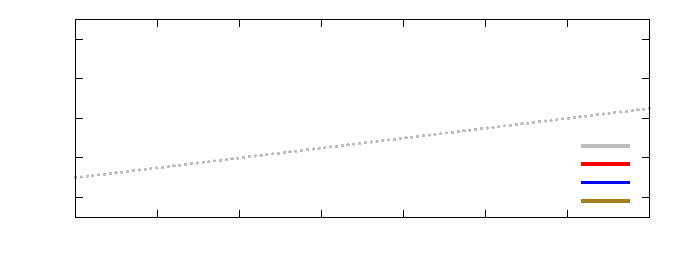
\includegraphics[width={453.00bp},height={170.00bp}]{chapters/results/image/Quinones}}%
    \gplfronttext
  \end{picture}%
\endgroup
